\documentclass[a4paper]{report}
\usepackage{geometry}
\usepackage[utf8]{inputenc}
\usepackage{graphicx}
\usepackage{fancyhdr}
\usepackage{amsmath}
\usepackage{amsfonts}
\usepackage{indentfirst}
\usepackage{amssymb}
\usepackage[T1]{fontenc}
\usepackage{array}
\usepackage{booktabs}
\usepackage[backend=biber,
style=numeric,
style=ieee
]{biblatex}
\addbibresource{reference.bib}

\graphicspath{ D:\\Learn\Uni\\ML\\CapstoneProject\\report\\figure }
\geometry{left=2.5cm, right=2.5cm, top=2cm, bottom=2cm}



\begin{document}
	
	\begin{titlepage}
		\centering
		
		\textsc{\textbf{HANOI UNIVERSITY OF SCIENCE AND TECHNOLOGY}}\\
		\textsc{\textbf{SCHOOL OF INFORMATION AND COMMUNICATION TECHNOLOGY}}\\[1.5cm]
		
		
		
\includegraphics[width= 0.7\textwidth]{logo-soict.png}\par\vspace{2cm}
		
		
		{\textsc{\Huge\bfseries{Project Report}} \\[0.5cm]}
		{\textsc{\LARGE \textbf{Stroke Risk Prediction}} \par}
		\vspace{1.5cm}
		
		\begin{center} \large
			\textbf{Course:} Machine Learning \\
			\textbf{Supervisor:} Assoc. Prof. Than Quang Khoat\\[1.5cm]
		\end{center}
		
		%\centering
		\begin{center} \large
			\begin{tabular}{l @{\hspace{3cm}} c}
				\emph{Authors:} & \emph{Student ID:} \\
				Nguyen Thanh An & 20225541 \\
				Pham Tuan Anh & 20225542 \\
				Le Tien Dat & 20225543 \\
				Nguyen Quang Hung & 20225545 \\
				Pham Doan Phuc Lam & 20225546 \\
				Le Hai Nhat & 20225583 \\
			\end{tabular}
		\end{center}
		
		\vfill
		
		{\large Hanoi, May 2024}
		
	\end{titlepage}
	
	\newpage
	\begin{center}
		{\fontsize{16pt}{20pt}\selectfont \textbf{Abstract}}\\
	\end{center}
	\paragraph{} \Large
	
	Stroke is a medical condition in which blood vessels in the brain rupture, causing brain damage. According to the World Health Organization (WHO), stroke is the leading cause of death and disability worldwide. Early recognition of stroke warning signs can help reduce the severity of stroke.
	
	Many machine learning (ML) models have been used to predict the likelihood of stroke occurrence. In this study, a dataset containing clinical and personal variables was used and several machine learning models were implemented to predict stroke and then to validate the results. The results highlight the significant importance of oversampling for imbalanced datasets like ours.
	\pagebreak
	
	\renewcommand*\contentsname{Table of contents}
	\tableofcontents
	
	
	
	\chapter*{\huge 1. Introduction} 
	\paragraph{}\Large
	A stroke is defined as an acute neurological disorder of the blood vessels in the brain that occurs when the blood supply to an area of the brain stops and the brain cells are deprived of the necessary oxygen. This can lead to brain cells dying within minutes, making stroke a medical emergency that requires immediate attention. Strokes can lead to severe disability or death, making an early detection and intervention crucial. 
	
	\paragraph{} \Large
	Factors that elevate the risk of having a stroke include a previous stroke, transient ischemic attacks, myocardial infarction, and other heart conditions such as heart failure and atrial fibrillation. Age is a significant factor; individuals over 55 are more likely to be affected, although strokes can occur at any age, including in children. Other risk factors are hypertension, carotid stenosis due to atherosclerosis, smoking, high cholesterol levels, diabetes, obesity, sedentary lifestyle, alcohol consumption, blood clotting disorders, estrogen therapy, and the use of substances like cocaine and amphetamines. 
	
	\paragraph{} \Large
	This project introduces a methodology for creating effective binary classification machine learning models for predicting stroke occurrence. Given the importance of class balancing for effective stroke prediction methods, the synthetic minority over-sampling technique (SMOTE) was utilized. Various models were then developed, configured, and evaluated on the balanced dataset. The models assessed included Naive Bayes, K-NN, decision trees, random forests, support vector machine (SVM), neural network and XG-boost. Additionally, majority voting and stacking methods were employed, with stacking being the main contribution of this study. The experiments demonstrated the superiority of the stacking method over single models and voting, achieving high precision, recall, F-measure, and accuracy.
	
	\addcontentsline{toc}{chapter}{\Large 1. Introduction}
	
	
	\chapter*{\huge 2. Data Set}
	\addcontentsline{toc}{chapter}{\Large 2. Dataset}
	
	\section*{\Large 2.1. Dataset description}
	\Large
	Our research based on a dataset from Kaggle \cite{dataset}. The original dataset has total 5110 participants, but here we take out randomly the data of 6 people for later testing. So our dataset now only has 5104 participants, and all of the attributes (10 as input to ML models and 1 for target class) are described as follows: 
	
	\begin{itemize} \Large
		\item \textbf{age}: Refers to participant's age.
		\item \textbf{gender}: Refers to participant's gender. The number of \emph{Male} is 2111. whilst the number of \emph{Female} is 2992 and 1 \emph{Other}.
		\item \textbf{hypertension}: Refers to whether participant has hypertension or not. \emph{1} for yes and \emph{0} for no.
		\item \textbf{heart\_disease}: Refers to whether participant has to suffer with heart disease. \emph{1} for yes and \emph{0} for no.
		\item \textbf{ever\_married}: Represents the marital status of the participants. \emph{Yes} or \emph{No}.
		\item \textbf{work\_type}: Represents the working status of participants. We have 5 categories ( \emph{children}, \emph{Govt\_job}, \emph{Never\_worked}, \emph{Private} or \emph{Self-employed}).
		\item \textbf{Residence\_type}: Represents where a person live, \emph{Rural} or \emph{Urban}.
		\item \textbf{avg\_glucose\_level}: Captures the participant's average glucose level.
		\item \textbf{bmi}: Represent the bmi of a person.
		\item \textbf{smoking\_status}: Captures the smoking status. (\emph{formerly smoked}, \emph{never smoked}, \emph{smokes} or \emph{Unknown}).
		\item \textbf{stroke}: Represents if the participant previously had a stroke or not.
		
	\end{itemize}
	\Large
	Except age, average\_glucose, bmi are numerical, most attributes are nominal.
	\addcontentsline{toc}{section}{\Large 2.1. Dataset description}
	
	\section*{\Large 2.2. Data Analysis and Preprocessing}
	\Large
	The following analysis shows a clear picture of how our dataset is. \\
	
	Figure 1 represents the distribution in attribute \textbf{stroke} (\emph{1} means the participant had a stroke in the past, while \emph{0} for not). With $4.8\%$ participants had stroke in the past, we can conclude that our data is highly unbalanced.
	
	\begin{center}
		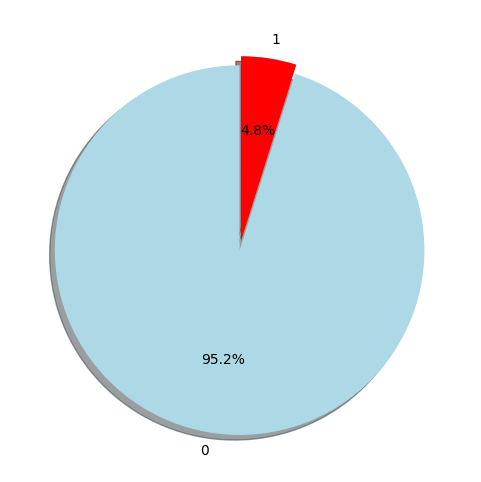
\includegraphics[scale=0.5]{imbalance.png} \\
		\small Figure 1. The distribution of stroke class
	\end{center}
	
	Figure 2 illustrates the distribution among work type and stroke class. We can see that people who work private and self-employed have higher chance of getting stroke, while people from government are more likely to not have a stroke. Moreover children and never worked participants are not very likely to get stroke. Maybe this could be explain due to the degree if pressure felt by workers.
	\begin{center}
		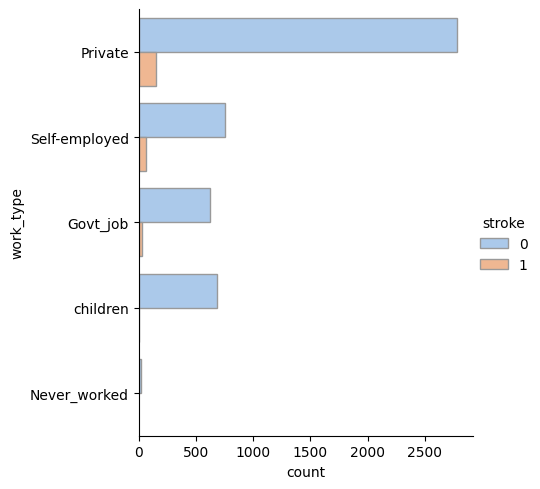
\includegraphics[scale=0.75]{work_type.png} \\
		\small Figure 2. The distribution among work type and stroke class
	\end{center}
	
	% section 2.2
	\addcontentsline{toc}{section}{\large 2.2. Data Analysis and Preprocessing}
	
	Figure 3 illustrates the distribution among smoking status and  stroke class. The stroke is not highly related to smokers, since the proportion of person having stroke is fairly the same among different status. 
	\begin{center}
		
		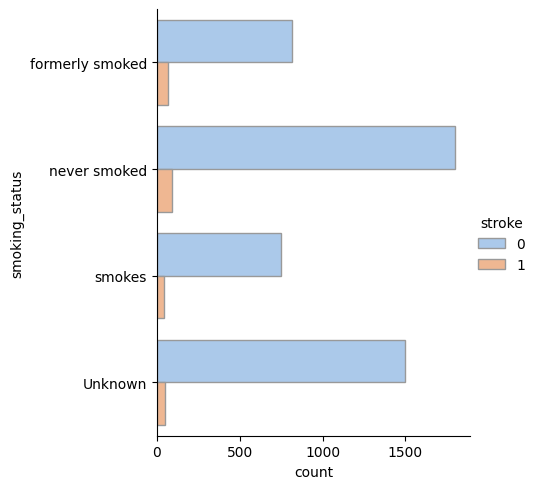
\includegraphics[scale=0.70]{smoke.png} \\
		\small Figure 3. The distribution among smoking status and stroke class
	\end{center} 
	\vspace{0.5cm}
	
	
	From the figure missing values \% in each columns, we can see that \textbf{bmi} is missing some data, at about 201 data. 
	\begin{center}
		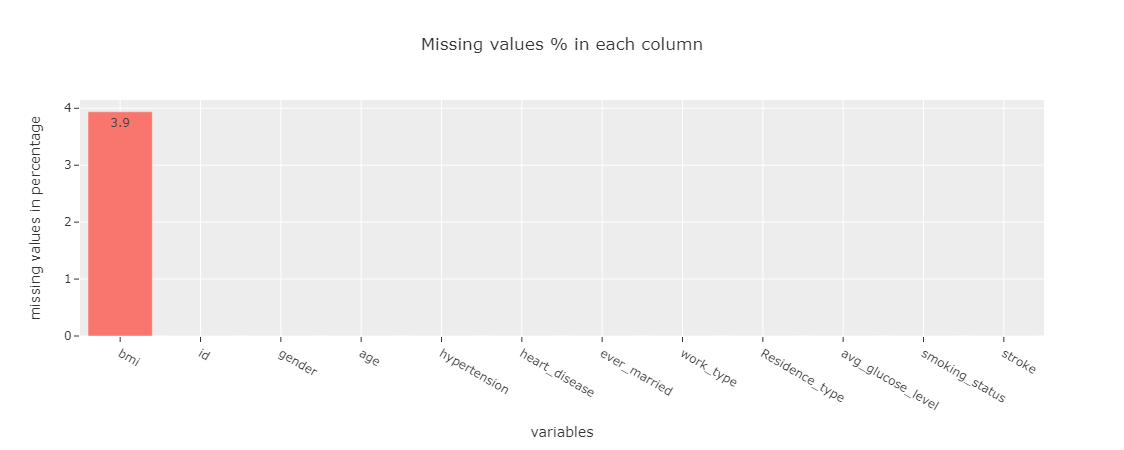
\includegraphics[scale=0.45]{missing_value.png}
	\end{center}
	
	To deal with missing data problem, we prefer to assign mean of bmi to these missing values. \\
	
	
	As can be seen from figure 1, our data is unbalanced. In our proposed framework, we employed a so-called SMOTE \cite{smote} to address the imbalanced distribution of participants among the stroke and non-stroke classes. More specifically, the minority class, in this case, the "stroke", was oversampled, such that the participants were equally distributed. In addition, after fixing the missing data problem, there were no more missing or null values, so neither dropping nor data imputation was further applied.
	% still section 2.2
	
	\chapter*{\huge 3. Proposed models} \Large
	\paragraph{}
	We present the models that will be utilized in the classification framework for stroke occurrence. For this purpose, several types of classifier are employed.
	\addcontentsline{toc}{chapter}{\Large 3. Proposed models}
	
	\section*{\Large 3.1. Bernoulli Naive Bayes} \Large
	\paragraph{}
	The Naive Bayes algorithm is a probabilistic classifier based on Bayes' Theorem. It assumes independence among features, making it simple yet effective for various tasks. Commonly used in text classification, spam detection, and sentiment analysis, it calculates the probability of each class given the input features. Despite its "naive" assumption of feature independence, it often performs well in practice, especially with large datasets. The model is fast, scalable, and easy to implement, making it a popular choice for many machine learning applications. \\
	
	\underline{\textbf{\Large Algorithm Overview}}
	\paragraph{}
	The probability calculations in Naive Bayes are influenced by the likelihood of the features. Therefore, there are three commonly used variants of Naive Bayes: Gaussian, Multinomial, and Bernoulli. The nature of the problem at hand will determine which variant is most suitable.
	
	For our problem of predicting stroke, we use Bernoulli Naive Bayes, suitable for continuous data, assuming that the features follow a Bernoulli distribution. Let c denotes the hypothesis that there is a stroke, and \( \overline{c} \) denotes the hypothesis that there is no stroke. Each X is composed of features \(x_1, x_2, x_3, \ldots, x_n\), which are the attributes or characteristics used to make the prediction, such as age, glucose levels, and body mass index (BMI).
	
	According to Bayes' theorem:
	
	\[P(c|X) = \frac{P(X|c)P(c)}{P(X)} \]
	
	\[P(\overline{c}|X) = \frac{P(X|\overline{c})P(\overline{c})}{P(X)} \] 
	where \( P(c|X) \) and \( P(\overline{c}|X) \) are posterior probabilities, \(P(X|c)\) and \(P(X|\overline{c})\) are likelihoods, \(P(c)\) and \(P(\overline{c})\) are class prior probabilities, and \(P(X)\) is predictor prior probabilities.
	
	To confirm whether we have a stroke or not, we compare \(P(c|X)\) and \(P(\overline{c}|X)\). More simply, we can compare \(P(X|c)P(c)\) and \(p(X|\overline{c})P(\overline{c})\). We have:
	\[P(X|c)P(c) = P(x_1|c) \times P(x_2|c) \times \ldots \times P(x_n|c) \times P(c)\]
	\[P(X|\overline{c})P(\overline{c}) = P(x_1|\overline{c}) \times P(x_2|\overline{c}) \times \ldots \times P(x_n|\overline{c}) \times P(\overline{c})\]
	
	\(P(c)\) is the proportion of stroke in training dataset, and \(P(\overline{c}) = 1 - P(c)\). 
	
	To determine \(P(x_i|c)\), we consider all the stroke in the training dataset, count the number of occurrences of \(x_i\) and divide it by the total number of patients.
	\[P(x_i|c) = \frac{N_cx_i}{N_c}\]
	
	\(P(x_i|\overline{c})\) is determined in the same way.\\
	
	\underline{\textbf{\Large Parameters}}
	
	\begin{itemize}
		\item \textbf{alpha}: It is a smoothing parameter used in the Naive Bayes algorithm. This parameter is to handle the problem of zero probabilities in the model.
		\item \textbf{binarize}: This parameter is used to threshold the feature values to binary values (0 or 1).
	\end{itemize}
	
	\underline{\textbf{\Large Choosing the suitable parameters}}
	\paragraph{}
	With default parameters on Bernoulli Naive Bayes classifier, we have following result:
	
	\begin{center}
		\begin{tabular}{ll}
			\toprule
			\textbf{Accuracy} & \textbf{75.78\%} \\
			\textbf{Precision}  & \textbf{72.14\%} \\
			\textbf{Recall}     & \textbf{83.81\%} \\
			\textbf{F1 score}   & \textbf{77.54\%} \\
			\bottomrule
		\end{tabular}
	\end{center}
	
	\paragraph{}
	Since default parameters show a temporary stable performance on metric scores, we perform a grid search over a range of hyperparameters to identify optimal values, using GridSearchCV class in Python's Scikit-learn library to automate this process. 
	
	The parameter grid is for this is: 
	\begin{verbatim}
		{"alpha" : [1.0, 1.25, 1.5, 1.75, 2.0], "binarize" = [0.0, 0.25, 0.5, 0.75, 1.0]}
	\end{verbatim}
	
	After performing the search, we found:
	\begin{verbatim}
		{"alpha" = 1.0, "binarize" = 0.5}
	\end{verbatim}
	
	We have following result:
	
	\begin{center}
		\begin{tabular}{ll}
			\toprule
			\textbf{Accuracy} & \textbf{76.04\%} \\
			\textbf{Precision}  & \textbf{72.26\%} \\
			\textbf{Recall}     & \textbf{84.33\%} \\
			\textbf{F1 score}   & \textbf{77.83\%} \\
			\bottomrule
		\end{tabular}
	\end{center}
	
	\paragraph{}
	However, after using the parameter, which is founded by GridSearchCV, the score of the model have no significant change. This problem maybe due to the lack of experiments involving other hyperparameters such as \texttt{"class\_prior"}, \texttt{"force\_alpha"}, \texttt{etc.}
	
	\addcontentsline{toc}{section}{\large 3.1. Bernoulli Naive Bayes}
	
	
	
	
	\section*{\Large 3.2. Support Vector Machine} \Large
	\paragraph{}
	A support vector machine (SVM) is a supervised machine learning algorithm that classifies data by finding an optimal line or hyperplane that maximizes the distance between each class in an N-dimensional space. It is one of the most popular and strong methods for classification since it can work well with very high dimensional problems.
	
	
	\paragraph{}
	\underline{\textbf{\textit{Types of SVM}}}
	
	\begin{itemize}
		\item \textbf{Linear SVM}:
		\paragraph{}
		Linear SVM is used for classification when the dataset is linear separable. The task is finding a hyperplane with max margin. There are two approaches to find that hyperplane.
		
		\begin{itemize}
			\item \textit{Hard-margin classification}: If the dataset is perfectly linear separable, hard-margin classification will provide accurate results. However, it is sensitive to noise.
			\item \textit{Soft-margin classification}: If the dataset is nearly linear separable, soft-margin classification will be applied. This method relaxes the constraint about the margin by using some slack variables, allowing for some misclassification to find reasonable results.
		\end{itemize}
		
		\item \textbf{Non-linear SVM}:
		\paragraph{}
		Much of the data in real-world scenarios are not linearly separable, and that’s where nonlinear SVM come into play. In order to make the data linearly separable, preprocessing methods are applied to the training data to transform it into a higher-dimensional feature space. That said, higher dimensional spaces can create more complexity by increasing the risk of overfitting the data and by becoming computationally taxing. The “kernel trick” helps to reduce some of that complexity, making the computation more efficient, and it does this by replacing dot product calculations with an equivalent kernel function.
		
		\paragraph{}
		Each kernel can be applied to different problems. Some of common kernel include:
		\begin{itemize}
			\item Linear kernel
			\begin{center}
				$k(x, z) = {x^T}z$
			\end{center} 
			\item Polynomial kernel
			\begin{center}
				$k(x, z) = (r + \gamma {x^T}z)^d$
			\end{center}
			\item Gaussian kernel
			\begin{center}
				$k(x, z) = \exp(-\gamma ||x-z||^2_2)$ ,\hspace{5mm} $\gamma > 0$
			\end{center}
			\item Sigmoid kernel
			\begin{center}
				$k(x, z) = \tanh(r + \gamma {x^T}z)$
			\end{center}
		\end{itemize}
	\end{itemize}
	
	\underline{\textbf{\large Models}}
	\paragraph{}
	In this project, we use 2 common kernels: \textit{linear} and \textit{Gaussian}
	\begin{itemize}
		\item For linear kernel: 
		\begin{itemize}
			\item $C$: Regularization parameter. The strength of the regularization is inversely proportional to C. We trained model with $C \in[0.1, 20]$.
		\end{itemize}
		\item For Gaussian kernel:
		\begin{itemize}
			\item $C \in [0.1, 20]$
			\item $\gamma \in [0.01, 1]$
		\end{itemize}
	\end{itemize}
	
	\pagebreak
	
	
	\textbf{\Large Linear Kernel}
	\paragraph{}
	Increasing value of C parameter resulted in long execution time. However, the accuracy score always around 78\%. The table below gives the result of linear kernel with $C = 1.0$.\\
	
	\begin{center}
		\begin{tabular}{ll}
			\toprule
			Accuracy Score & 78.20\% \\
			Precision Score & 75.62\% \\
			Recall Score & 83.79\% \\
			F1 Score & 79.50\% \\
			\bottomrule
		\end{tabular}
	\end{center}
	\begin{center}
		Result of linear kernel with $C = 1.0$
	\end{center}
	
	\textbf{\Large Gaussian Kernel}
	\paragraph{}
	After training, the most feasible values are $C = 3.0$ and $\gamma = 0.2$. The table below gives the result.
	
	\begin{center}
		\begin{tabular}{ll}
			\toprule
			Accuracy Score & 95.78\% \\
			Precision Score & 96.19\% \\
			Recall Score & 95.40\% \\
			F1 Score & 95.79\% \\
			\bottomrule
		\end{tabular}
	\end{center}
	
	\begin{center}
		Result of Gaussian kernel with $C = 3.0$ and $\gamma = 0.2$
	\end{center}
	
	\addcontentsline{toc}{section}{\large 3.2. Support Vector Machine}
	
	
	
	\section*{\Large 3.3. Decision Tree and Random Forest} \Large
	\addcontentsline{toc}{section}{\large 3.3. Decision Tree and Random Forest} 
	
	\subsection*{3.3.1. Decision Tree} \Large
	\paragraph{}
	A tree-like model of decision and their possible consequences, including chance event outcomes, resource cost, and utility. \\
	
	\underline{\textbf{\Large Parameters}}
	\begin{itemize} 
		\item \textbf{criterion}: Here we specify which method we will choose when performing split operations. Partition is the most important concept in decision trees. It is very crucial to determine how to split and when to split.
		\item \textbf{splitter}: It is the strategy of how to split node.
		\item \textbf{max\_feature}: The number of features to consider when splitting, We can determine the maximum number of features to be used by giving integers and proportionally by giving float number.
	\end{itemize}
	
	\underline{\textbf{\Large Choosing the suitable parameters}}\\[0.5cm]
	With default hyperparameters on Decision Tree classifier, we have following result:
	
	\begin{center}
		\begin{tabular}{ll}
			\toprule
			\textbf{Accuracy score} & \textbf{91.20\%} \\
			\textbf{Precision score}  & \textbf{90.57\%} \\
			\textbf{Recall score}     & \textbf{92.14\%} \\
			\textbf{F1 score}   & \textbf{91.35\%} \\
			\bottomrule
		\end{tabular}
	\end{center}
	
	\paragraph{}
	Default parameters show a good performance on metric scores, but we still perform a grid search over a range of hyperparameters to identify optimal values, using GridSearchCV class in Python's scikit-learn library to automate this process. The parameter grid is for this is: \\
	
	\begin{verbatim}
		{"criterion" : ["gini" , "entropy", "log_loss"], 
			"splitter" : ["best", "random"], 
			"max_features" : ["auto", "sqrt", "log2"]}
	\end{verbatim}
	
	
	After performing the search, we found:
	\begin{verbatim}
		"criterion": "log_loss", "max_features": "log2", "splitter": "best"
	\end{verbatim}
	With following table result:
	
	\begin{center}
		\begin{tabular}{ll}
			\toprule
			\textbf{Accuracy score} & \textbf{89.81\%} \\
			\textbf{Precision score}  & \textbf{88.94\%} \\
			\textbf{Recall score}     & \textbf{91.12\%} \\
			\textbf{F1 score}   & \textbf{90.02\%} \\
			\bottomrule
		\end{tabular}
	\end{center}
	
	However, after using founded parameter, the score of the model is lower than the score of default parameter. This may be due to the lack of experiments involving other hyperparameters such as "max\_depth", "max\_leaf\_node", .etc...
	
	\addcontentsline{toc}{subsection}{\normalsize 3.3.1. Decision Tree}
	
	
	
	\subsection*{3.3.2. Random Forest Classifier} \Large
	\paragraph{}
	Random Forest (RF) \cite{RF} ensembles many independent decision trees and, by resampling, creates different subsets of instances to perform classification and regression tasks. Each decision tree exports its own classification outcome, and then the final class is derived through majority voting. 
	
	\underline{\textbf{\Large Parameters}}
	\begin{itemize} 
		\item \textbf{criterion}: Here we specify which method we will choose when performing split operations. Partition is the most important concept in decision trees. It is very crucial to determine how to split and when to split.
		\item \textbf{max\_feature}: The number of features to consider when splitting, We can determine the maximum number of features to be used by giving integers and proportionally by giving float number.
	\end{itemize}
	
	\underline{\textbf{\large Choosing the suitable parameters}}\\[0.5cm]
	With default hyperparameters on Random Forest classifier, we have following result:
	
	\begin{center}
		\begin{tabular}{ll}
			\toprule
			\textbf{Accuracy score} & \textbf{95.06\%} \\
			\textbf{Precision score}  & \textbf{94.07\%} \\
			\textbf{Recall score}     & \textbf{96.20\%} \\
			\textbf{F1 score}   & \textbf{95.12\%} \\
			\bottomrule
		\end{tabular}
	\end{center}
	
	\paragraph{}
	Default parameters show a good performance on metric scores, but we still perform a grid search over a range of hyperparameters to identify optimal values, using GridSearchCV class in Python's scikit-learn library to automate this process. The parameter grid is for this is:
	\begin{verbatim}
		{'max_depth': [10, 20, 30, 40, 50, 60, 70, 80, 90, 100],
			'criterion' :[ 'gini' , 'entropy','log_loss'],
			'max_features': ['auto', 'sqrt', 'log2']} 
	\end{verbatim}
	
	After performing the search, we found:
	\begin{verbatim}
		{"criterion"="log_loss", "max_features"="sqrt", "max_depth"=100}
	\end{verbatim} 
	
	\begin{center}
		\begin{tabular}{ll}
			\toprule
			\textbf{Accuracy} & \textbf{93.98\%} \\
			\textbf{Precision}  & \textbf{92.22\%} \\
			\textbf{Recall}     & \textbf{96.39\%} \\
			\textbf{F1 score}   & \textbf{94.26\%} \\
			\bottomrule
		\end{tabular}
	\end{center}
	
	Similar to decision tree, we experienced a worse result. However the recall is higher is higher, but it is negligible. 
	
	\addcontentsline{toc}{subsection}{\normalsize 3.3.2. Random Forest Classifier}
	
	\section*{\Large 3.4. K-nearest Neighbors}
	\paragraph{} \Large
	K-Nearest Neighbors (KNN) is a popular versatile machine learning algorithm used for both classification and regression tasks. It's known for its simplicity, ease of implementation, and interpretability. KNN works by classifying (or predicting) data points based on the labels of their nearest neighbors in the training data. The number of neighbors considered is a crucial parameter, denoted by "k". \\
	
	\underline{\textbf{\Large Classifying with KNN}}
	
	\paragraph{}
	Given with a dataset with labeled instances, KNN classifies new instances by analyzing the labels of its closest neighbors in the training data. To \textit{Analyze} the labels of its \textit{k} nearest neighbors, model determine distances from current instance to others. Then analyze labels of each instances.\\
	
	\underline{\textbf{\Large{Parameters}}}
	\begin{itemize}
		\item \textbf{K (Number of Neighbors)}: The value of \textit{K} significantly impacts KNN's performance. Experimenting with different k values using techniques like cross-validation is crucial to find the optimal k for your dataset.
		\item \textbf{Distance Metric}: is a function used to determine the similarity or "closeness" between two data points. KNN relies on this distance metric to identify the k nearest neighbors of a new data point for classification or regression tasks. Here are some common distance metrics used in KNN:\begin{itemize}
			\item \textbf{Euclidean Distance}: This is the most widely used metric. It calculates the straight-line distance between two points in n-dimensional space. Imagine points plotted on a graph - Euclidean distance is the familiar distance formula used to find the length of that line.
			\[
			\scalebox{2.0}{$\sqrt{\sum_{i=1}^{n}(\mathnormal{x}_i  - \mathnormal{y}_i)^2}$}
			\]
			\item \textbf{Manhattan Distance}: Also known as the L1 norm or city block distance, it calculates the total distance traveled along each dimension to get from one point to another.
			\[
			\scalebox{2.0}{$\sum_{i=1}^{n} | \mathnormal{x}_i - \mathnormal{y}_i |$}
			\]
			\item \textbf{Cosine Similarity}: This metric is often used for text data or high-dimensional data. It reflects the cosine of the angle between two data points. Intuitively, a higher cosine similarity indicates a more similar direction between the points.
			\[
			\scalebox{2.0}{$\frac{\sum_{i=1}^{n}\mathnormal{x}_i \times \mathnormal{y}_i }{ \sqrt{\sum_{i=1}^{n}{\mathnormal{x}_i}^2}  \times \sqrt{\sum_{i=1}^{n}{\mathnormal{y}_i}^2}}$}
			\]
		\end{itemize}
		\item \textbf{Weighting Neighbors}: it refers to assigning different importance to the k nearest neighbors identified for a new data point. By default, KNN treats all k neighbors equally. However, weighting allows you to prioritize closer neighbors and give them more influence in the final prediction.
	\end{itemize}
	\pagebreak
	
	\underline{\textbf{\Large{Choosing suitable parameters}}}
	
	\paragraph{}
	
	The value of K is crucial because it determines how many neighbors influence the prediction for a new data point. With a too small k, The model becomes oversensitive to noise in the training data and may not capture the underlying patterns well. Imagine a noisy neighborhood - a small k might focus on the closest neighbors, even if they're noisy outliers. Besides, a too large k can lead model be underfitting and the model might lose sight of the local patterns and become overly generalized. After iterating k from 1 to 30 and examining the performance of model, I sum up this below graph.\\
	
	
	\begin{figure}[th]
		\centering
		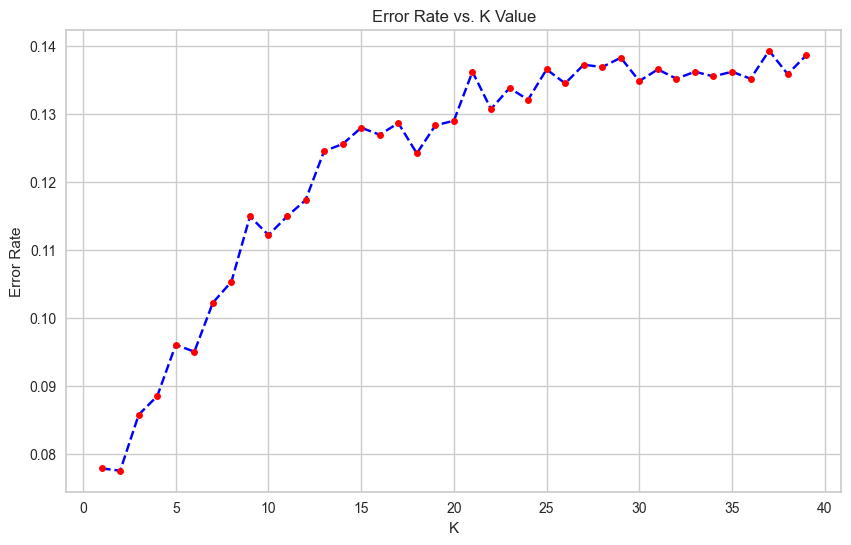
\includegraphics[scale=0.6]{error_rate.png}
		\caption{Experimental error rate with each k neighbors}
		\label{fig:enter-label}
	\end{figure}
	
	After analyzing above graph, larger k is equivalent to larger error rate. And we can see that when k = 2 the error rate is smallest. Here is model's score:
	
	\begin{center}
		\begin{tabular}{ll}
			\toprule
			\textbf{Accuracy score} & 92.21\% \\
			\textbf{Precision score} & 91.56\%\\
			\textbf{Recall score} & 92.84\% \\
			\textbf{F1 score } & 92.20\%\\
			\bottomrule
		\end{tabular}
		
		\label{tab:example}
	\end{center}
	\begin{center}
		Test result for optimal value k = 2
	\end{center}
	After finding optimal value for k, I perform a grid search over a range of hyperparameters to identify other optimal values, using the GridSearchCV class that has been installed within Python's scikit-learn library to automate this process. The parameter grid is : 
	\begin{verbatim}
		"neighbors" : [1, 30], 
		"metric" : ["euclidean", "manhattan", "cosine"], 
		"weights": ["uniform", "distance"]
	\end{verbatim}
	Grid search return the following parameters
	\begin{verbatim}
		"neighbors"=1, "metric"="manhattan", "weights": "uniform"
	\end{verbatim}
	with result:
	\begin{center}
		\begin{tabular}{ll}
			\toprule
			\textbf{Accuracy score} & 92.38\% \\
			\textbf{Precision score} & 89.33\%\\
			\textbf{Recall score} & 96.04\% \\
			\textbf{F1 score } & 92.56\%\\
			\bottomrule
		\end{tabular}
	\end{center}
	But we have an optimal k (neighbors value) = 2, while grid search return optimal k = 1, so we test our model again with:
	\begin{verbatim}
		"neighbors"=2, "metric"="manhattan", "weights": "uniform"
	\end{verbatim}
	and we received the result:
	\begin{center}
		\begin{tabular}{ll}
			\toprule
			\textbf{Accuracy score} & 92.86\% \\
			\textbf{Precision score} & 92.01\%\\
			\textbf{Recall score} & 93.67\% \\
			\textbf{F1 score } & 92.83\%\\
			\bottomrule
		\end{tabular}
	\end{center}
	Overall, this is better than the above two cases.
	\addcontentsline{toc}{section}{\large 3.4. K-nearest Neighbor}
	
	\section*{\Large 3.5. Logistic Regression}
	\Large
	\paragraph{}
	Logistic regression accomplishes binary classification task by predicting the probability of an outcome, event, or observation. In context of stroke risk prediction, it attempts to determine whether a participant has higher chance to get stroke or not.
	
	\underline{\textbf{\Large Parameters}}\\
	
	L1 and L2 regularization are techniques used to prevent overfitting in machine learning models. We continue to use the GridSearchCV to find the suitable parameters among:
	\begin{verbatim}
		"solver": ["lbfgs", "liblinear"],
		"max_iter": [100, 200, 300, 400, 500], 
		"multi_class": ["auto", "ovr", "multinomial"], 
		"penalty": ["l1", "l2", "elasticnet", "none"],
	\end{verbatim} 
	The optimal parameters we found are 
	\begin{verbatim}
		"solver"="lbfgs", "max_iter"=200, 
		"multi_class"="auto", penalty"="l2"
	\end{verbatim}
	with the following result:
	\begin{center}
		\begin{tabular}{ll}
			\toprule
			\textbf{Accuracy score} & 75.76\% \\
			\textbf{Precision score} & 75.58\%\\
			\textbf{Recall score} & 76.88\% \\
			\textbf{F1 score } & 76.22\%\\
			\bottomrule
		\end{tabular}
	\end{center}
	\begin{center}
		Test result for tuning Logistic Regression
	\end{center}
	\addcontentsline{toc}{section}{\large 3.5. Logistic Regression}
	
	\section*{\Large 3.6. XGBoost}
	\addcontentsline{toc}{section}{\large 3.6. XGBoost}
	
	\paragraph{}
	XGBoost \cite{XGBoost}, which stand for Extreme Gradient Boosting, based on gradient boosting. However, it comes with great improvements in algorithm optimization and the perfect combination of software and hardware power, helping to achieve outstanding results in both training time and memory used. \\
	
	\underline{\textbf{\Large{Parameters}}}
	
	\begin{itemize}
		\item \textbf{n\_estimators}: Determines the number of boosting iterations and controls the overall complexity of the model.
		\item \textbf{learning\_rate}: An optimal parameter where step size shrinkage prevents overfitting.
		\item \textbf{booster}: 
		\item \textbf{gamma}: L1 regularization term on weights
		\item \textbf{reg\_lambda}: L2 regularization term on weights.
		%\item \textbf{base\_score}: 
	\end{itemize}
	
	\underline{\textbf{\Large Choosing suitable parameters}}
	
	Similar to other methods, we first run the model with default parameters:
	
	\begin{center}
		\begin{tabular}{ll}
			\toprule
			\textbf{Accuracy score} & \textbf{94.49\%} \\
			\textbf{Precision score}  & \textbf{92.75\%} \\
			\textbf{Recall scorer}     & \textbf{96.63\%} \\
			\textbf{F1 score}   & \textbf{94.65\%} \\
			\bottomrule
		\end{tabular}
	\end{center}
	
	\paragraph{}
	We keep using GridSearchCV to automate identify the optimal values for the hyperparameters. The grid for this is: 
	\begin{verbatim}
		{"n_estimators": [100, 500, 1000], "learning_rate"': [0.01, 0.1, 0.5],
			"booster": ["gbtree", "gblinear"], "gamma": [0, 0.5, 1], 
			"reg_lambda": [0, 0.5, 1]}
	\end{verbatim}
	\paragraph{}
	The optimal parameters we found is 
	\begin{verbatim}
		{"booster"="gbtree", "gamma"=0, "learning_rate"=0.1,
			"n_estimator"=1000, "reg_lambda"=0}
	\end{verbatim} 
	
	With following table result:
	
	\begin{center}
		\begin{tabular}{ll}
			\toprule
			\textbf{Accuracy score} & \textbf{95.57\%} \\
			\textbf{Precision score}  & \textbf{95.00\%} \\
			\textbf{Recall score}     & \textbf{96.18\%} \\
			\textbf{F1 score}   & \textbf{95.59\%} \\
			\bottomrule
		\end{tabular}
	\end{center}
	
	
	\addcontentsline{toc}{chapter}{\Large 4. Results}
	\chapter*{\huge 4. Results}
	\section*{\Large 4.1. Evaluation metrics}
	\paragraph{} \Large
	Under the evaluation process of the considered ML models, several performance metrics were recorded. In this project, we have used some commonly metrics.
	
	Denote:
	\begin{itemize}
		\item TP: the number of true positives
		\item TN: the number of true negatives
		\item FP: the number of false positives
		\item FN: the number of false negatives
	\end{itemize}
	We evaluate the performance of our system based of the following criteria 
	
	\begin{itemize}
		\item \textit{Accuracy} =  $ \displaystyle \frac{TP + TN}{TP + TN + FP + FN}$
		\item\textit{Precision} = $\displaystyle\frac{TP}{TP + FP}$
		\item \textit{Recall} = $\displaystyle\frac{TP}{TP + FN}$
		\item \textit{F1 score} = $\displaystyle 2 \times \frac{\text{Precision} \times \text{Recall}}{\text{Precision} + \text{Recall}}$
	\end{itemize}
	
	\addcontentsline{toc}{section}{\large 4.1. Evaluation metrics}
	\pagebreak
	
	\section*{\Large 4.2. Compare results}
	Performance among different models
	
	\renewcommand{\arraystretch}{1.5} % Adjust row spacing
	
	\begin{tabular}{|c|c|c|c|c|}
		\toprule
		& \textbf{Accuracy} & \textbf{Precision} & \textbf{Recall} & \textbf{F1} \\
		\hline
		\textbf{Naive Bayes} & 76.04\% & 72.26\% & 84.33\% & 77.83\% \\
		\textbf{SVM (Linear)}   & 78.20\% & 75.62\% & 83.79 \% & 79.50\% \\
		\textbf{SVM (Gaussian)}  & 95.78\% & 96.19\% & 95.40\% & 95.79\% \\
		\textbf{Decision Tree}    & 91.20\% & 90.57\% & 92.14\% & 91.35\% \\
		\textbf{Random Forest}    & 95.06\% & 94.07\% & 96.20\% & 95.12\% \\
		\textbf{KNN Classifier}    & 92.86\% & 92.01\% & 93.67\% & 92.83\% \\
		\textbf{Logistic Regression}    & 75.76\% & 75.58\% & 76.88\% & 76.22\% \\
		\textbf{XGBoost}    & 95.57\% & 95.00\% & 96.18\% & 95.59\% \\
		\bottomrule
	\end{tabular}
	\begin{center}
		\textit{Performance of different models}
	\end{center}
	Except Naive Bayes, SVM (linear kernel) and Logistic regression show poor performance, the other models show amazing performance (over 91\%).
	
	\paragraph{}
	Random Forest, SVM(Gaussian kernel) and XGBoost illustrate the best performance, at around 95\%. There are a few differences in their recall score and precision score. SVM (Gaussian kernel) is the finest since its accuracy score and f1-score was the highest, at \textbf{95.78\%} and \textbf{95.79\%}, respectively.
	
	\addcontentsline{toc}{section}{\large 4.2. Compare results}
	
	\chapter*{\huge 5. Conclusions}
	A stroke constitutes a threat to a human’s life that should be prevented and/or treated to avoid unexpected complications. Nowadays, with the rapid evolution of AI/ML, the clinical providers, medical experts and decision-makers can exploit the established models to discover the most relevant features (or risk factors) for the stroke occurrence, and can assess the respective probability or risk.
	
	In this direction, machine learning can aid in the early prediction of stroke and mitigate the severe consequences. This study investigates the effectiveness of various ML algorithms to identify the most accurate algorithm for predicting stroke based on several features that capture the participants’ profiles.
	
	The performance evaluation of the classifiers using F-measure (which summarizes precision and recall) and accuracy is essentially suitable for the models’ interpretation, demonstrating their classification performance. In addition, they reveal the models’ validity and predictive ability in terms of the stroke class. Support Vector Machine with Gaussian kernel classification outperforms the other methods, with an F1-score of 95.79\% and an accuracy of 95.78\%. Hence, a SVM (Gaussian) is an efficient approach for identifying those at high risk of experiencing a stroke in the long term.
	\addcontentsline{toc}{chapter}{\Large 5. Conclusions}
	
	
	\chapter*{\huge \centering REFERENCES}
	\printbibliography[heading=none]
	\addcontentsline{toc}{chapter}{\Large REFERENCES}
	\newpage
\end{document}          
